\section{Data Preprocessing and feature selection}

\subsection{Missing Value Imputation}

The dataset contains 9105 rows and 48 columns with varying degrees of missingness(Figure \ref{fig:missing_distribution}).:

\begin{itemize}
    \item \textbf{Target Variable (\texttt{sfdm2}):} Missing in 1400 rows (15.38\%). These rows were removed to avoid data leakage, as imputing the target variable would undermine model integrity.
    \item \textbf{Predictor Variables:} 32 variables had missing values, with some exceeding 50\% (e.g., \texttt{adlp}, \texttt{urine}).
\end{itemize}

\begin{figure}[!h]
\centering
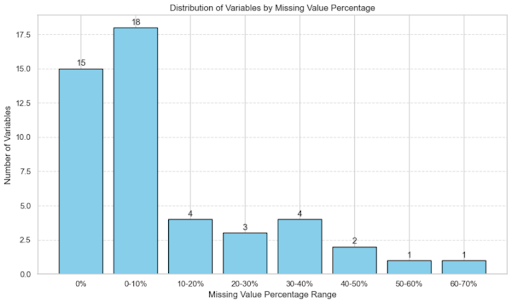
\includegraphics[width=0.8\textwidth]{../results/missing_distribution.png}
\caption{Distribution of missing values in the dataset}
\label{fig:missing_distribution}
\end{figure}

To address missing values, we employed a combination of clinical imputation and custom imputation pipelines. 
The imputation process was designed to ensure that the data remained representative and suitable for modeling.

\begin{enumerate}
    \item \textbf{Clinical Imputation:} We used reference values from the dataset documentation to impute 7 clinical variables:
    \begin{itemize}
        \item \texttt{alb}: 3.5, \texttt{pafi}: 333.3, \texttt{bili}: 1.01, \texttt{crea}: 1.01, \texttt{bun}: 6.51, \texttt{wblc}: 9.0, \texttt{urine}: 2502
    \end{itemize}
    
    \item \textbf{Custom Imputation Pipelines:} We designed three imputer types tailored to the data types:
    \begin{table}[H]
    \centering
    \caption{Imputation Strategy Table}
    \begin{tabular}{|c|c|c|}
    \hline
    \textbf{Imputer Type} & \textbf{Variable Feature} & \textbf{Imputation Methods} \\
    \hline
    I   & Numerical        & Mean, Median, Constant, KNN \\
    II  & Categorical      & One-hot: Most frequent, Constant \texttt{Unknown} \\
    III & Categorical      & Simple: Most frequent, Constant \texttt{Unknown} \\
    \hline
    \end{tabular}
    \end{table}
\end{enumerate}

By combining the methods in each imputer type, we generated 16 distinct
imputed datasets (4 $\times$ 2 $\times$ 2) to enable comparative modeling.


\begin{figure}[!h]
\centering
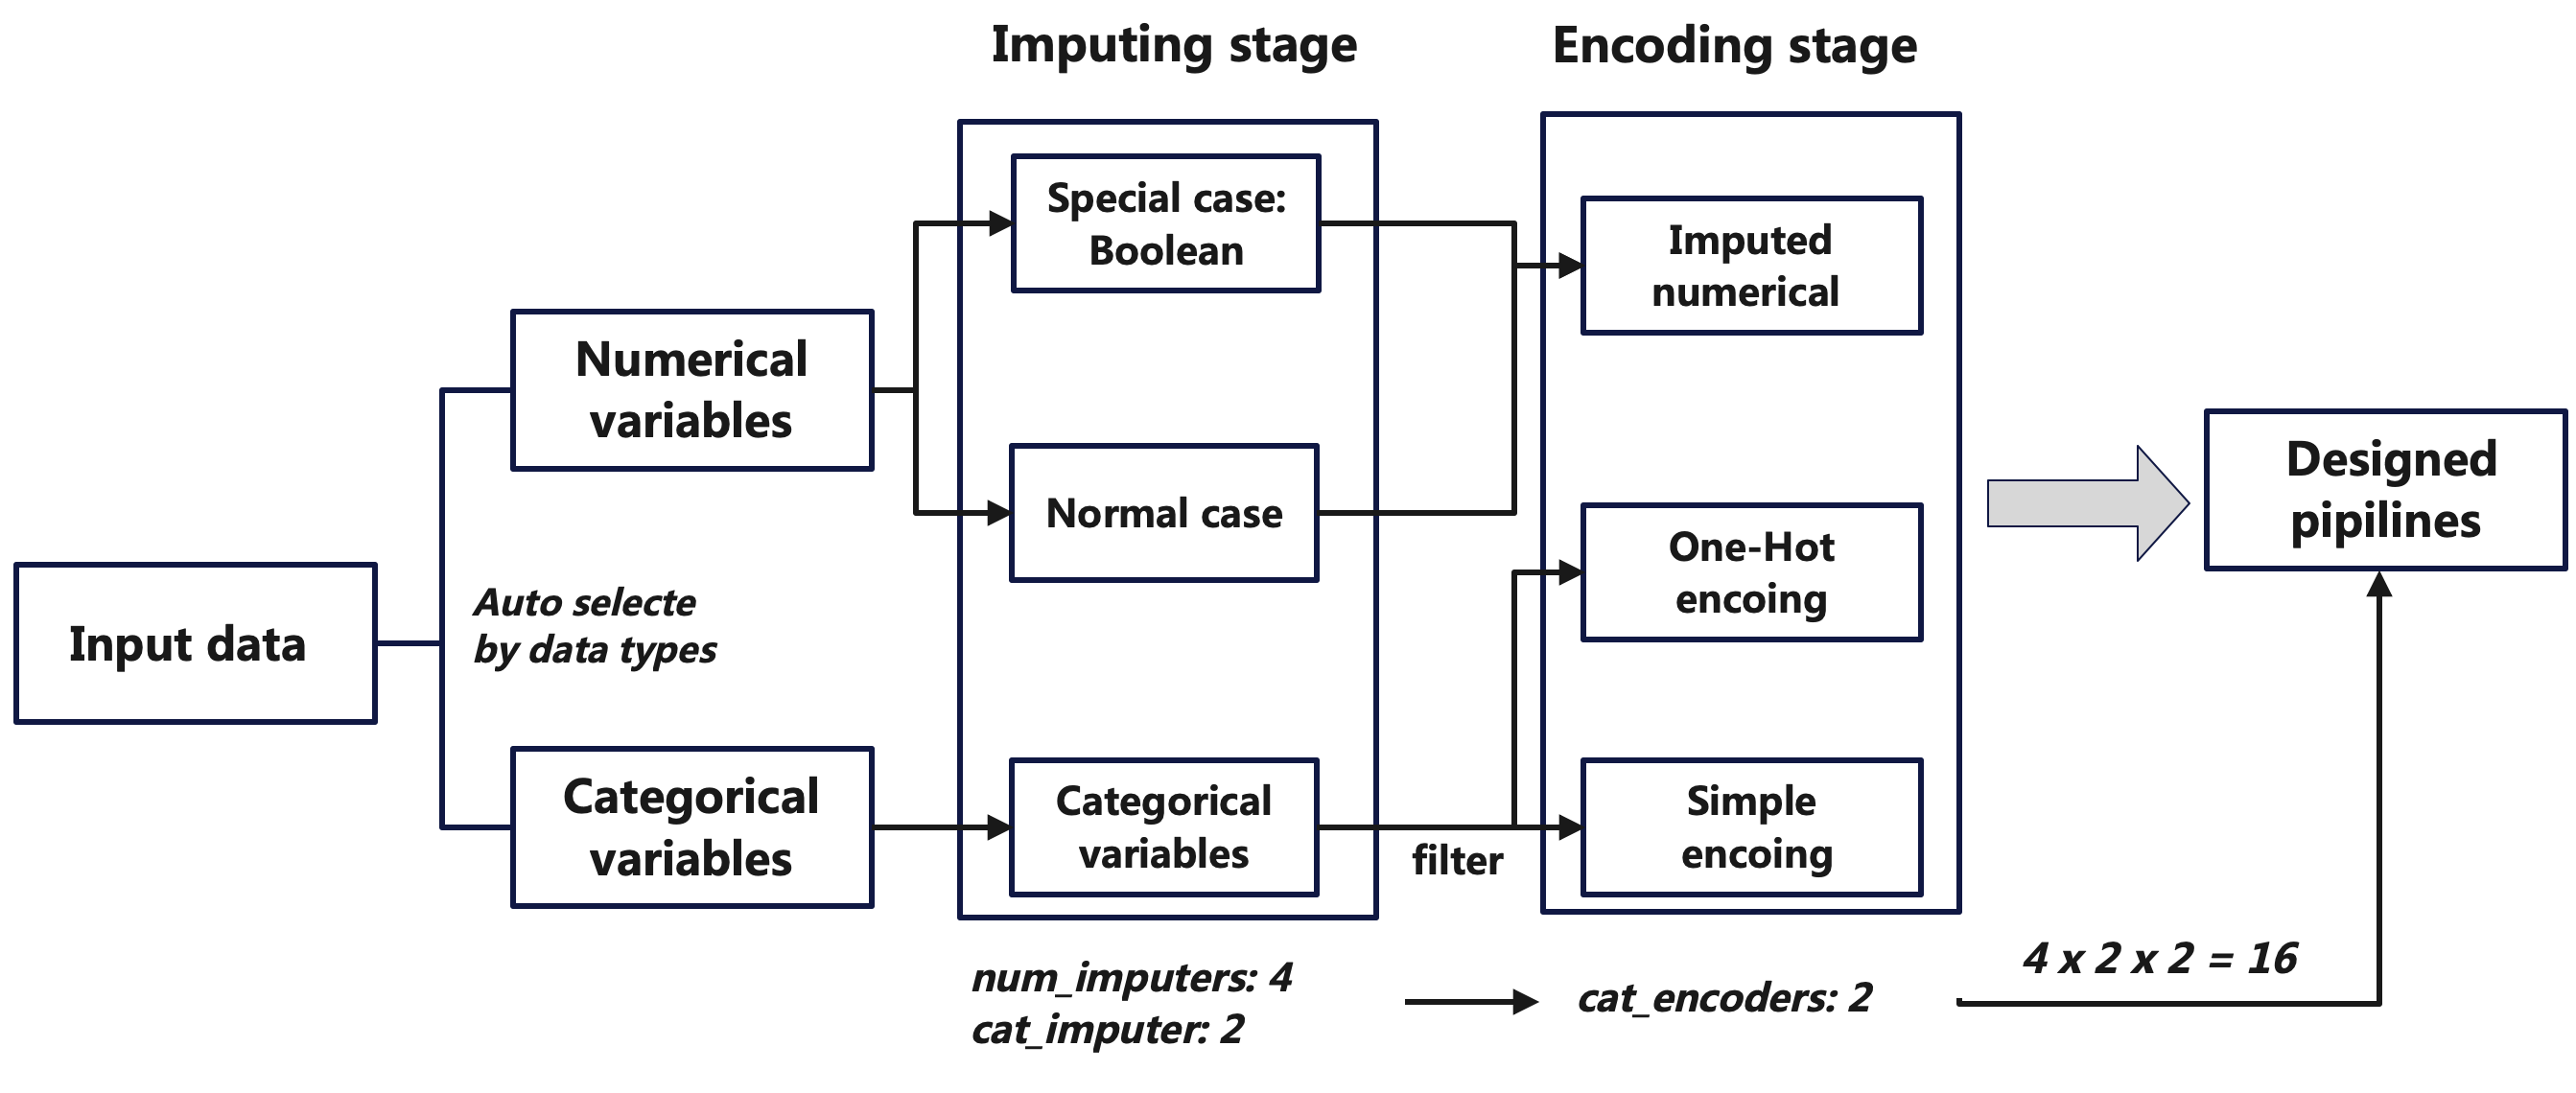
\includegraphics[width=0.8\textwidth]{../results/pipeline_imputing.png}
\caption{Design of Imputation Pipelines}
\label{fig:imputation_pipeline}
\end{figure}

\textbf{Simple Encoding:} For certain qualitative variables, 
simple imputation methods are not directly applicable due to their ordinal nature and
the arbitrary encoding generated by default functions. 
To address this, we established a custom mapping scheme for these variables,
as detailed in Table \ref{tab:encoding_mapping}.


\begin{table}[H]
    \centering
    \caption{Simple Encoding Mapping('--' indicates no mapping)}
    \label{tab:encoding_mapping}
    \begin{tabular}{|c|c|c|c|}
    \hline
    \textbf{Encoded} & \textbf{Income} & \textbf{DNR} & \textbf{SFDMS (sfdm2)} \\
    \hline
    0 & Unknown & Unknown & -- \\
    1 & Under \$11k & No DNR & No (Month 2 and SIP present) \\
    2 & \$11k-\$25k & DNR after SADM & ADL $\geq$ 4 (5 if survived) \\
    3 & \$25k-\$50k & DNR before SADM & SIP $\geq$ 30 \\
    4 & \>\$50k & -- & Coma or Intub \\
    5 & -- & -- & $<$ 2 mo. follow-up \\
    \hline
    \end{tabular}
\end{table}

\textbf{One-Hot Encoding:} Applied to multi-class categorical variables where 
the order of categories is not meaningful,
such as \texttt{sex}, \texttt{dzgroup}, and \texttt{dzclass}.


\subsection{Data Leakage Mitigation}

To ensure model generalizability, we removed variables that could leak information about the outcome:

\begin{itemize}
    \item \texttt{death}, \texttt{hospdead}, \texttt{slos}, \texttt{d.time} — these variables represent outcomes or timing after the 2-month period and can leak post-prediction information into training.
    \item Inclusion of these variables may indirectly reveal mortality and discharge timing, violating the principle that only pre-outcome data be used for prediction.
\end{itemize}

\subsection{Stratified Train-Test Split}

We performed an 80/20 split of the dataset, using stratified sampling to preserve the distribution of the \texttt{sfdm2} outcome variable.
Standardization was applied to all features to reduce outlier influence and ensure consistent data scale.

\textcolor{red}{fig in appendix}

\section{Feature Selection}

\section{Multiple Logistic Regression}

We applied MLR to each of selected sub datasets to identify the most accurate imputation strategy. The model predicts:
\[
P(Y = 1 \mid X) = \frac{e^{\beta_0 + \sum_{j=1}^{p} \beta_j X_j}}{1 + e^{\beta_0 + \sum_{j=1}^{p} \beta_j X_j}}
\]
where \( \beta_j \) are the coefficients estimated through log-likelihood maximization.

\subsection{LASSO Regularization}

We used Lasso regression to select the most important features from the dataset, and use the selected features to build the model.
The optimization problem for Lasso regression can be formulated as:

\[
\hat{\beta} = \arg\min_{\beta} \left\{ \frac{1}{n} \sum_{i=1}^n \left( y_i - \mathbf{x}_i^\top \beta \right)^2 + \lambda \sum_{j=1}^p |\beta_j| \right\}
\]

The reason we chose lasso instead of ridge is that the lasso penalty, \( \lambda \sum_{j=1}^p |\beta_j| \), encourages sparsity in the coefficients, 
which drop some of coefficients to zero when some features are highly correlated(shown in Figure \ref{fig:correlation_matrix}). However, ridge regression will not 
drop the highly correlated features, but will give them similar coefficients, which does not help to reduce the model complexity.

We tuned $\lambda$ using a stratified 5-fold cross-validation over a log-transformed range: $\log(1/\lambda)$ from $[-4, 2]$.

\subsection{Choosing of selected features and best imputation strategy}

We evaluated model performance across the 16 imputation pipelines:
\begin{itemize}
    \item \textbf{Best Imputation Strategy:} Imputer-2 achieved the highest accuracy of \textbf{71.87\%}.
    \item \textbf{Optimal} \( \lambda = 0.033598 \), selected using 5-fold cross-validation.
\end{itemize}

The final LASSO model retained 23 predictors, balancing interpretability with predictive strength.

For model simplicity, we selected the 14 most important predictors based 
on their significance in the LASSO regression result and their contribution to predicting \texttt{sfdm2}.

\begin{figure}[!h]
\centering
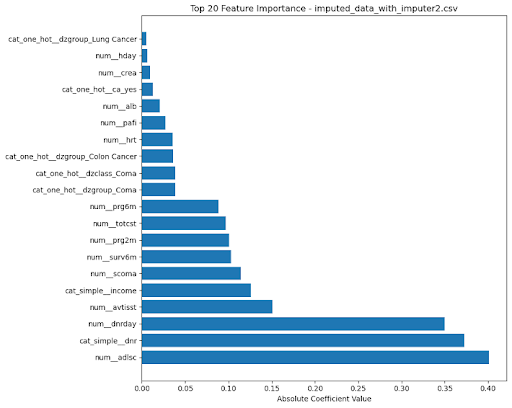
\includegraphics[width=0.8\textwidth]{../results/feature_selected_Lasso.png}
\caption{Rank of feature importantce in LASSO model}
\label{fig:feature_importance}
\end{figure}